% Copyright 2004 by Till Tantau <tantau@users.sourceforge.net>.
%
% In principle, this file can be redistributed and/or modified under
% the terms of the GNU Public License, version 2.
%
% However, this file is supposed to be a template to be modified
% for your own needs. For this reason, if you use this file as a
% template and not specifically distribute it as part of a another
% package/program, I grant the extra permission to freely copy and
% modify this file as you see fit and even to delete this copyright
% notice. 

\documentclass{beamer}

% There are many different themes available for Beamer. A comprehensive
% list with examples is given here:
% http://deic.uab.es/~iblanes/beamer_gallery/index_by_theme.html
% You can uncomment the themes below if you would like to use a different
% one:
%\usetheme{AnnArbor}
%\usetheme{Antibes}
%\usetheme{Bergen}BEMS-SoftwareArchitecture
%\usetheme{Berkeley}
%\usetheme{Berlin}
%\usetheme{Boadilla}
%\usetheme{boxes}
%\usetheme{CambridgeUS}
%\usetheme{Copenhagen}
%\usetheme{Darmstadt}
%\usetheme{default}
%\usetheme{Frankfurt}
%\usetheme{Goettingen}
%\usetheme{Hannover}
%\usetheme{Ilmenau}
%\usetheme{JuanLesPins}
%\usetheme{Luebeck}
\usetheme{Madrid}
%\usetheme{Malmoe}
%\usetheme{Marburg}
%\usetheme{Montpellier}
%\usetheme{PaloAlto}
%\usetheme{Pittsburgh}
%\usetheme{Rochester}
%\usetheme{Singapore}
%\usetheme{Szeged}
%\usetheme{Warsaw}


% Customize Warsaw color 
\setbeamercolor*{palette primary}{use=structure,fg=white,bg=red!50!black}
\setbeamercolor*{palette secondary}{use=structure,fg=white,bg=red!60!black}
\setbeamercolor*{palette tertiary}{use=structure,fg=white,bg=red!70!black}

% Customize Warsaw block title and background colors
\setbeamercolor{block title}{bg=red!50!black,fg=white}


% List your packages here

\usepackage[colorinlistoftodos]{todonotes}


\title[Progress Update]{A Generalized Open Source Platform for Building Energy Management}

% % A subtitle is optional and this may be deleted
% \subtitle{Product Proposal}

\author[B.~Lauer]{Brian~Lauer\\\and
Advisor: Dr. Suruz Miah}
% - Give the names in the same order as the appear in the paper.
% - Use the \inst{?} command only if the authors have different
%   affiliation.

\institute[Bradley University] % (optional, but mostly needed)
{
  Department of Electrical and Computer Engineering\\
  Bradley University\\
  1501 W. Bradley Avenue\\
  Peoria, IL, 61625, USA
}
% - Use the \inst command only if there are several affiliations.
% - Keep it simple, no one is interested in your street address.

\date[June~11,~2020]{Thursday, June~11,~2020}
% - Either use conference name or its abbreviation.
% - Not really informative to the audience, more for people (including
%   yourself) who are reading the slides online

\logo{\hfill\href{http://www.bradley.edu}{
\includegraphics[width=0.75cm]{../figs/logoBU1-Print}}}  % place logo in every page 


\subject{Mobile Robot Localization}
% This is only inserted into the PDF information catalog. Can be left
% out. 

% If you have a file called "university-logo-filename.xxx", where xxx
% is a graphic format that can be processed by latex or pdflatex,
% resp., then you can add a logo as follows:

% \pgfdeclareimage[height=0.5cm]{university-logo}{university-logo-filename}
% \logo{\pgfuseimage{university-logo}}

% Delete this, if you do not want the table of contents to pop up at
% the beginning of each subsection:

% Let's get started
\begin{document}

\begin{frame}
  \titlepage
\end{frame}

\begin{frame}{Outline}
  \tableofcontents
  % You might wish to add the option [pausesections]
\end{frame}

% Section and subsections will appear in the presentation overview
% and table of contents.
\section{Introduction}

\begin{frame}{Introduction}{}
  % applications of mobile robot navigation and problem description
  \begin{figure}
  	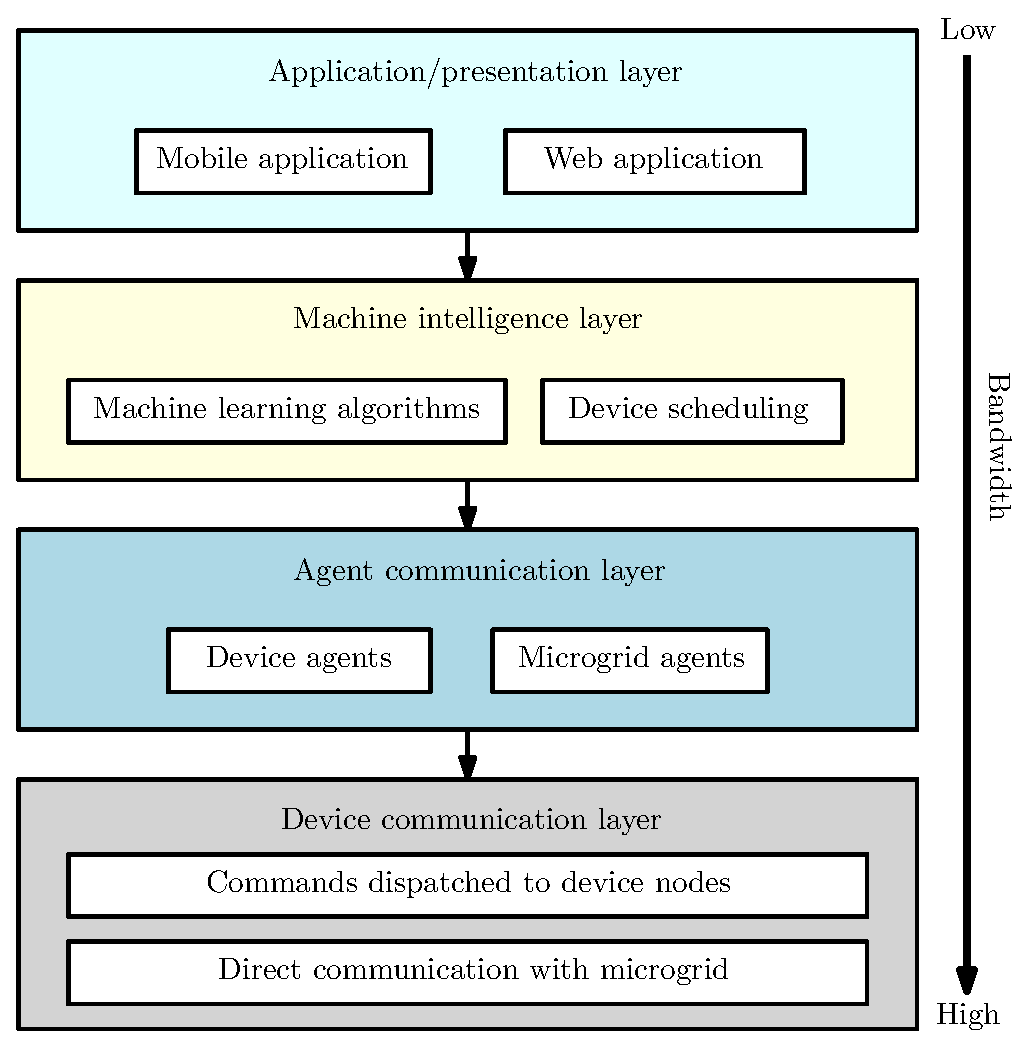
\includegraphics[scale=0.35]{../figs/ipe/BEMS-softwareArchitecture}
  \end{figure}
\end{frame}

\begin{frame}{Introduction}{}
	\begin{figure}
		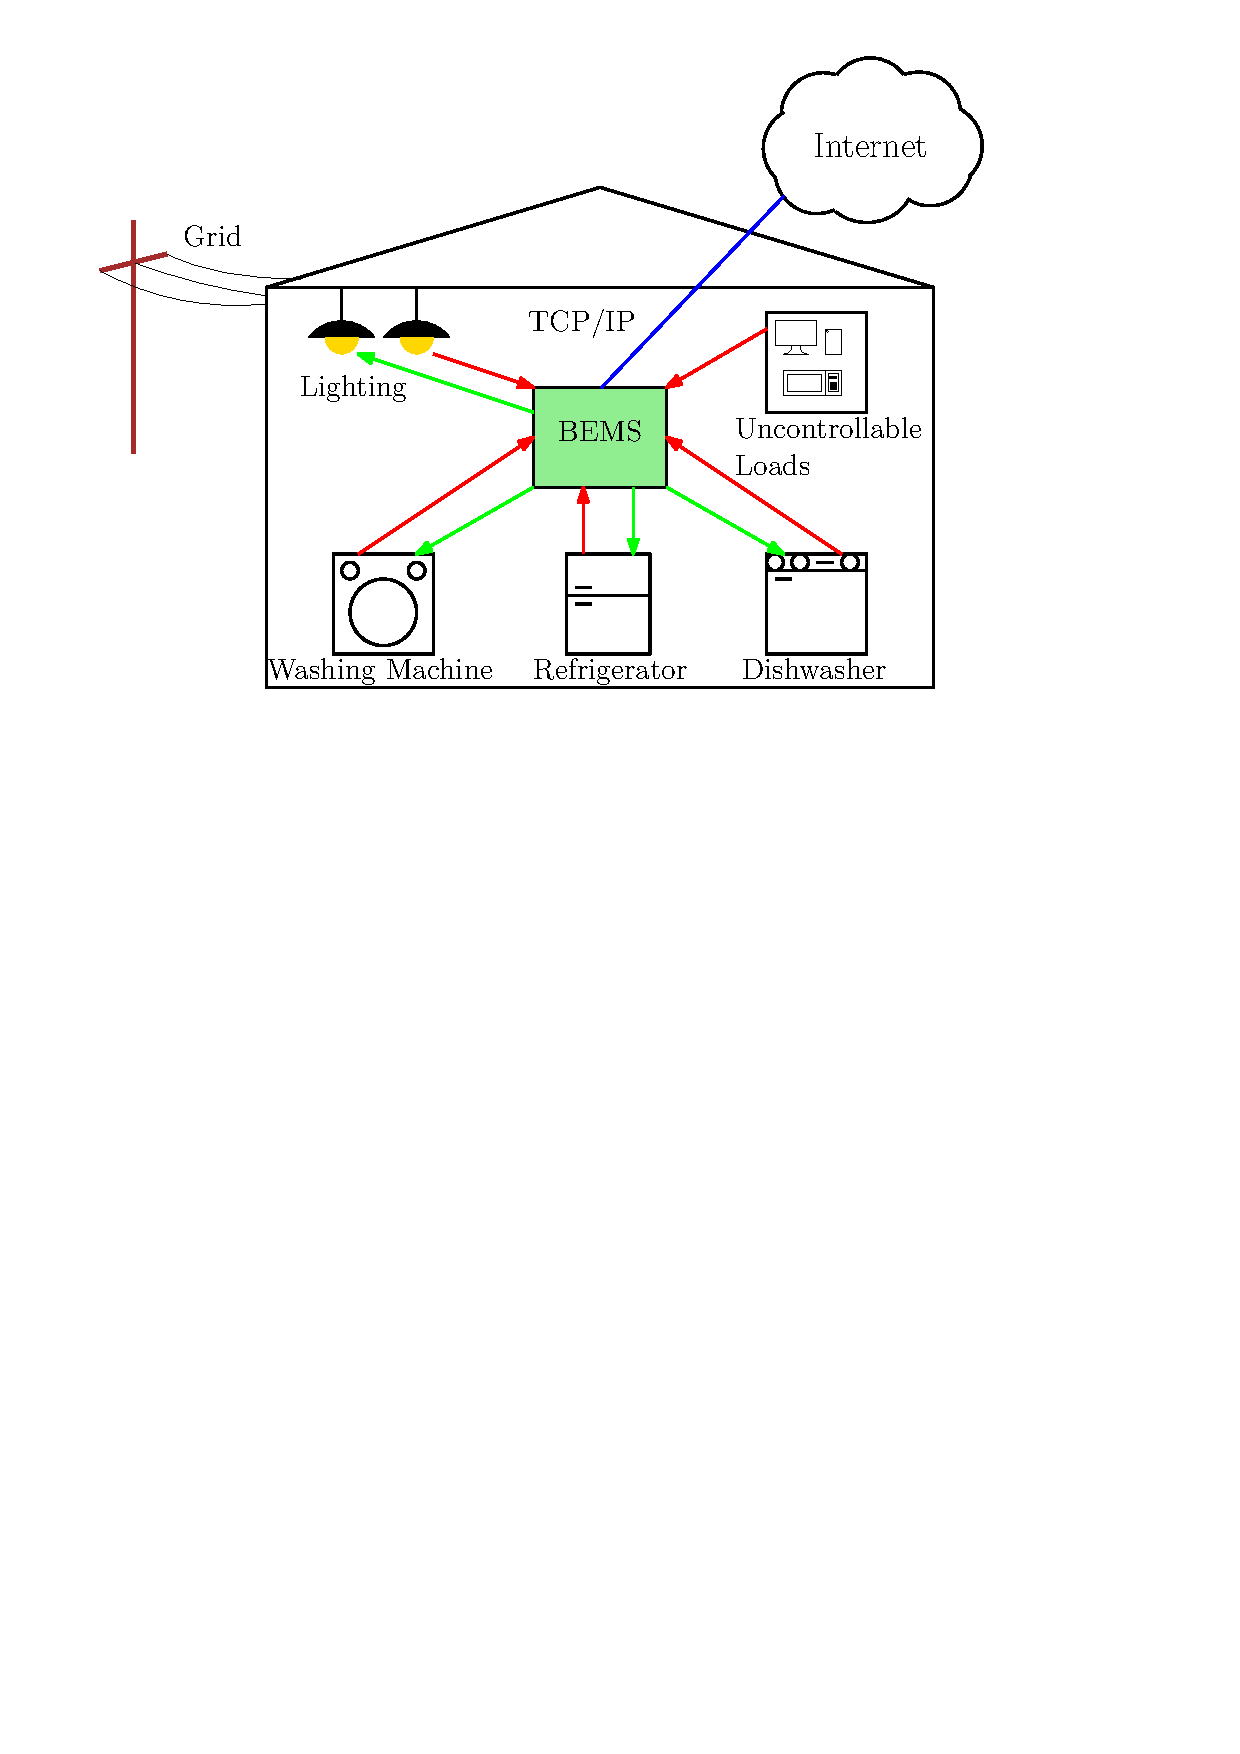
\includegraphics[scale=0.4]{../figs/ipe/bemsdiagram}
	\end{figure}
\end{frame}

\section{Progress}
\begin{frame}{Progress}{}
\begin{itemize}
	\item Wrote method \texttt{setDeviceToActive} to add a discovered device to the list of Active Devices once it is discovered by the \texttt{DiscoveryAgent} class
	\item Added a modal popup to, in the future, show the recently discovered devices
	\item Started reading \textit{Federated Reinforcement Learning for Energy Management of Multiple Smart Homes with Distributed Energy Resources}
\end{itemize}
\end{frame}

\section{Progress}
\begin{frame}{Progress}{}
\begin{figure}
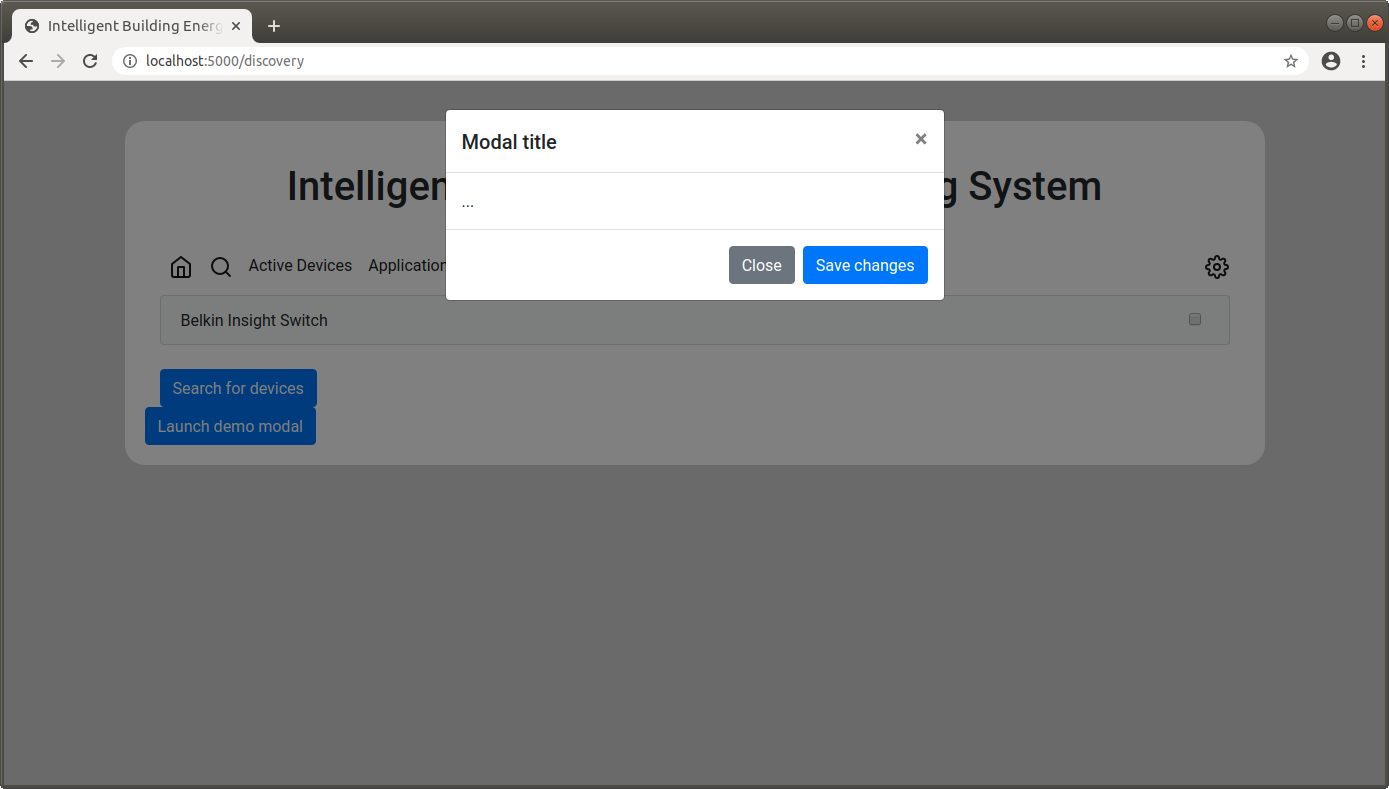
\includegraphics[scale=0.2]{../figs/img/modalView}
\caption{View of discovered devices page with modal popup}
\end{figure}
\end{frame}
%----------------------------------

\section{Plans}
\begin{frame}{Plans}{}
\begin{itemize}
\item Need to connect the DiscoveryAgent to the discovery page to let the server know when to enable the popup
\item Start work on the active devices page
\item Finish reading the paper 
\end{itemize}
\end{frame}

% You can reveal the parts of a slide one at a time
% with the \pause command:
%\begin{frame}{Second Slide Title}
%  \begin{itemize}
%  \item {
%    First item.
%    \pause % The slide will pause after showing the first item
%  }
  %\item {   
  %  Second item.
 % }
  % You can also specify when the content should appear
  % by using <n->:
 % \item<3-> {
 %   Third item.
 % }
%  \item<4-> {
%    Fourth item.
 % }
  % or you can use the \uncover command to reveal general
  % content (not just \items):
%  \item<5-> {
%    Fifth item. \uncover<6->{Extra text in the fifth item.}
%  }
%  \end{itemize}
%\end{frame}

%\section{Second Main Section}

%\subsection{Another Subsection}

%\begin{frame}{Blocks}
%\begin{block}{Block Title}
%You can also highlight sections of your %presentation in a block, with it's own %title
%\end{block}
%\begin{theorem}
%There are separate environments for %theorems, examples, definitions and proofs.
%\end{theorem}
%\begin{example}
%Here is an example of an example block.
%\end{example}
%\end{frame}

% Placing a * after \section means it will not show in the
% outline or table of contents.s



% All of the following is optional and typically not needed. 
\appendix
\section<presentation>*{\appendixname}
\subsection<presentation>*{For Further Reading}

\begin{frame}[allowframebreaks]

  \frametitle<presentation>{References}
    
  \begin{thebibliography}{10}
    
  \setbeamertemplate{bibliography item}[online]
  
  \bibitem{bootstrap}
  Bootstrap
  \newblock \url{https://getbootstrap.com/https://getbootstrap.com/}
  \end{thebibliography}
\end{frame}

\end{document}



%%% Local Variables:
%%% mode: latex
%%% TeX-master: t
%%% End:
